\section{Evaluation}
\label{sec:evaluation}

\subsection{Case Study: Developing a SVM for traffic sign detection}

For the case study scikit-learn \cite{scikit-learn} and for preparation of the dataset in Python OpenCV2 have different function to load and resize images \cite{opencv_library}. In their work, Stallkamp et al. \cite{DBLP:conf/ijcnn/StallkampSSI11} built a mulit-category classification dataset. The mulit-category classification dataset contains german traffic signs for image classification. That mulit-category classification dataset uses the german traffic signs from a approx. 10 hours daytime video from different roads.

\subsection{The original dataset preparation}

The original dataset from Stallkamp et al. is splitted between a training and testing folder. The training folder separate 42 signs into subfolders. The information of the folders are written in an eponymous csv-file that are not needed further in this case study. In Figure \ref{fig:traffic_signs} the traffic sign names (a) - (f) are the labels for this present case study.

\begin{figure}[h!]
  \centering
  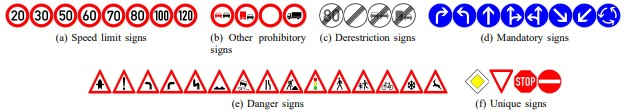
\includegraphics[width=12cm]{pictures/traffic_signs.jpg}
  \caption{Labeled traffic signs \cite{DBLP:conf/ijcnn/StallkampSSI11}}
  \label{fig:traffic_signs}
\end{figure}

All signs are resized to 300x300 pixel and are flattened for a higher efficiency.

\subsection{Differences between manipulated and original dataset}
